\subsection{Effetto del materiale sulla misura}

Abbiamo testato quanto la presenza di lastre di metallo potesse influire sulla rivelazione dei raggi cosmici,
per indagare quanto possa essere rilevante il materiale circostante (soffitto, pareti).
Abbiamo a disposizione:
\begin{itemize}
	\item 3 lastre di piombo rivestite di alluminio, ciascuna di spessore totale \SI{4}{mm},
	\item 1 lastra di alluminio di spessore \SI{4}{mm},
	\item 10 lastre di piombo spesse \SI{2}{mm}.
\end{itemize}
Non abbiamo misurato lo spessore della parte di piombo di quelle con piombo e alluminio.
Le lastre di metallo ricoprono circa l'\SI{80}\% delle lastre di scintillatore. 

\subsubsection{Conteggi}

\begin{table}
\centering
\begin{tabular}{| c | r @{\,$\pm$\,} l | r @{\,$\pm$\,} l | r @{\,$\pm$\,} l |}
\hline
$\#$lastre & \multicolumn{2}{c|}{$C3$} & \multicolumn{2}{c|}{$C2$} & \multicolumn{2}{c|}{$C3/C2$} \\ 
\hline
0 & 13455&116 & 20248&142 & 0.664&0.003 \\
1 & 13328&115 & 20381&143 & 0.654&0.003 \\
2 & 13400&116 & 20438&143 & 0.655&0.003 \\
4 & 12715&113 & 20071&142 & 0.633&0.003 \\
\hline
\end{tabular}
\caption{Dati presenti nel grafico di \autoref{cfr}.}
\label{dati cfr}
\end{table}

\begin{figure}
\centering
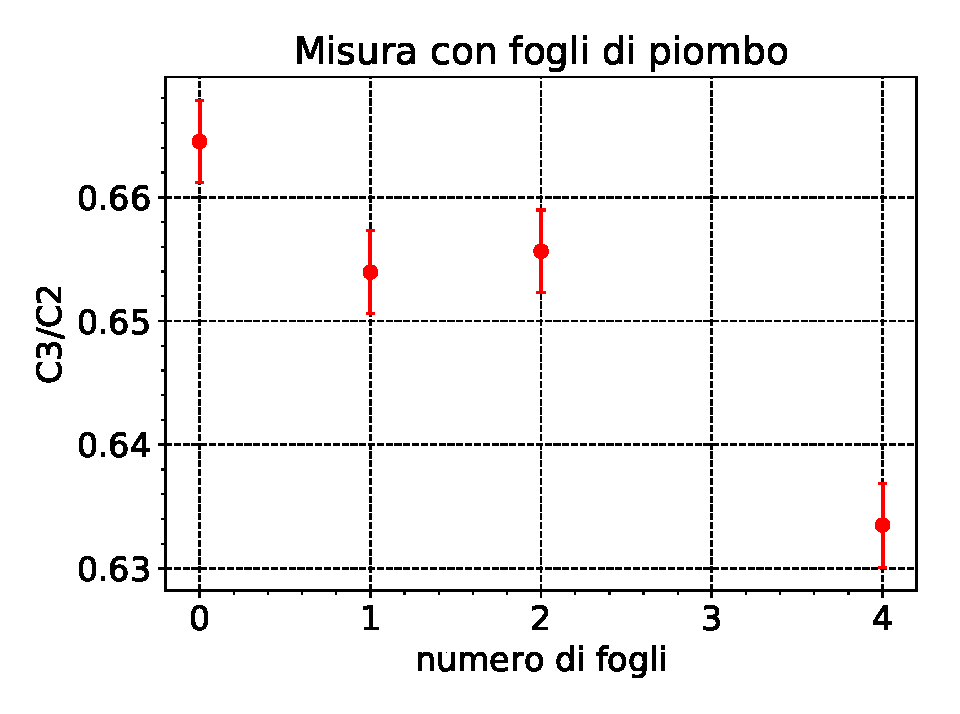
\includegraphics[width=8 cm]{confronto}
\caption{Rapporto tra coincidenze a 3 ($C3$) e coincidenze a 2 ($C2$) in funzione delle lastre di materiale inserite.}
\label{cfr}
\end{figure}

Abbiamo posizionato le lastre di metallo tra il PM3 ed il PM4
per vedere se esse riuscivano a fermare parte dei raggi cosmici.

Per fare questa misura abbiamo confrontato il rapporto tra le coincidenze 5\&4\&3 e 5\&4
al variare del numero di lastre di metallo.
Abbiamo confrontato i rapporti per non dover tener conto dell'accettanza%
\footnote{Sia l'efficienza che la geometria.}.
L'errore sui rapporti è dato dalla formula
$$ \sigma(C3/C2)= \sqrt{ \frac{C3/C2\cdot (1-C3/C2)}{C2} } $$
che descrive la deviazione standard di un rapporto tra coincidenze in cui si tiene conto della correlazione tra gli eventi in coincidenza a 3 e quelli in coincidenza a 2. La dimostrazione di tale formula è presente in \autoref{sec:vareff}.

La \autoref{cfr} evidenzia un assorbimento di particelle da parte del piombo: si tratta probabilmente degli elettroni che sono riusciti ad attraversare il tetto\footnote{Sospettiamo che il 2\si{\degree} e 3\si{\degree} rapporto siano compatibili perché la lastra aggiunta era d'alluminio.}.

\subsubsection{Energia}

Infine abbiamo eseguito due acquisizioni di lunga durata.
Nella prima abbiamo messo tutte le lastre a nostra disposizione sul PM1
e abbiamo acquisito i loro rilasci di energia per tutta la notte.
Il giorno seguente le abbiamo tolte ed abbiamo preso dati per \SI{4}{ore}.
In entrambi i casi il trigger dell'ADC è dato dalle coincidenze PM2 \& PM1.

\begin{figure}
	\hspace{-10em}
	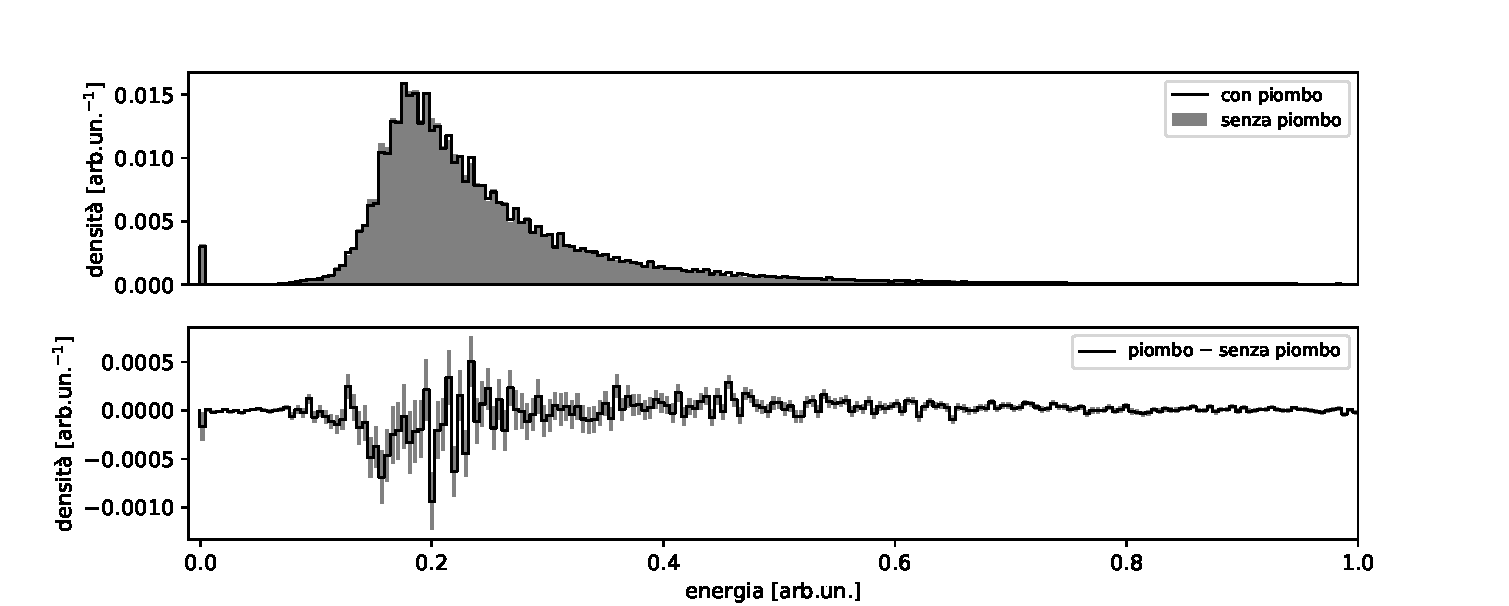
\includegraphics[width=1.6\textwidth]{piombo_energia}
	\caption{\label{fig:piomboenergia}
		Distribuzione del rilascio di energia sul PM1 con e senza lastre di piombo.
		Ogni bin contiene 6 digit dell'ADC.
		Il secondo grafico riporta la differenza delle due distribuzioni con le incertezze.}
\end{figure}

Il risultato è riportato in \autoref{fig:piomboenergia}.
Dal grafico della differenza delle distribuzioni
si nota che la distribuzione con il piombo è spostata verso energia maggiore.
È in effetti plausibile che le particelle rallentate dal piombo
rilascino più energia a causa della risalita di ionizzazione.
Per verifica confrontiamo i due campioni con il test di Kolmogorov-Smirnov a $5\sigma$,
risulta significativo.
